\documentclass[11pt]{article}
\usepackage{enumitem}
\usepackage{float}
\usepackage[margin=1in]{geometry}
\usepackage{graphicx}
\usepackage[space]{grffile}
\usepackage{adjustbox}
\usepackage{amsmath}
\usepackage{amsthm}
\usepackage{amssymb}
\usepackage{fullpage}
\usepackage{fancyhdr}
\usepackage{xparse}
\newcommand*{\boxtex}[1]{\framebox{#1}}
\newcommand{\cnum}{CM146}
\newcommand{\ced}{Fall 2018}
\newcommand{\ctitle}[3]{\title{\vspace{-0.5in}\cnum, \ced\\Problem Set #1: #2}}
\newcommand{\solution}[1]{{{\color{blue}{\bf Solution:} {#1}}}}
\NewDocumentCommand{\texcod}{mm}{%
	\texttt{\textcolor{#1}{#2}}%
}
\usepackage[usenames,dvipsnames,svgnames,table,hyperref]{xcolor}

\renewcommand*{\theenumi}{\alph{enumi}}
\renewcommand*\labelenumi{(\theenumi)}
\renewcommand*{\theenumii}{\roman{enumii}}
\renewcommand*\labelenumii{\theenumii.}

\author{Zheng Wang}
\date{\today}
\title{MATH 151A Homework 1}

\begin{document}
\maketitle

\section*{Question 1}
\begin{itemize}
	\item[(a)]
	We will first show there is at least one solution for $ f(x)=0 $. \\\\
	 Notice that $ f(0.5) = -0.1 < 0 $ and $ f(1) = 0.3 > 0 $. Also, since $ f(x) $ is a polynomial function, so it is continous for $ x \in \mathbb{R} $, so $ f(x) $ is continous $ \forall x \in [0.5,1] $. By Intermediate Value Theorem, since $ f(0.5) < 0 < f(1) $, it follows that there exist some $ \xi \in  (0.5,1) $ such that $ f(\xi) = 0 $.\\\\
	We then show that $ \xi $ is unique.\\\\
	We find that $ f'(x) = 2x-0.7 $ is a continous function for all $ x \in \mathbb{R} $. Thus for $ x \in [0.5,1] $, $ f'(x) \in [0.3,1.3] $. Suppose that there exist more than one solution for the equation $ f(x)=0 $, then we have $ f(\xi)=f(\xi')=0 $, where $ \xi \ne \xi' $. Therefore, since $ f(x) $ is continous, differentiable on $ (\xi,\xi') $ (without loss of generality, assume that $ \xi < \xi' $), and $ f(\xi) = f(\xi')=0 $, by Rolle's Theorem, there exist some $ x^* \in (\xi, \xi') $ such that $ f'(x^*) = 0 $, a contradiction. \hfill$ \blacksquare $ 
	
	\item[(b)]
	Claim: $ \left| p_n- p \right| \le \frac{1-0.5}{2^n}  $.\\
	\textit{proof.} Since $ b_n - a_n = \frac{1}{2}(b_{n-1} - a_{n-1}) = \frac{1}{2^{n-1}}(b_1 - a_1) $. Also, since $ p_n = \frac{1}{2} (a_n+b_n) $.
	
	Thus, \[ \left| p_n - p \right| \le \frac{1}{2}\left(b_n-a_n \right) = \frac{1}{2^n}(b_1-a_1) = \frac{1-0.5}{2^n} \]
	\hfill$ \blacksquare $
	
	Thus, to have $ p_k - p \le 10^{-5} $, we must have $ 10^{-5} \ge \frac{1-0.5}{2^k} $. By solving the equation, we have $ k \ge \frac{5}{\log{2}} -1 \approx 15.6 $. Therefore, we must take \boxtex{$ k = 16 $} steps then the error will be less than $ 10^{-5} $. \pagebreak
	
	
\end{itemize}
\section*{Question 2}
Take $ g(x) = f(x)-x $. Then if $ g(x) = 0 $, $ f(x) = x $. There are two cases for $ f(x) $, we will discuss them one by one.
\subsection*{Case 1}
If $ f(a) = a$ or $ f(b) = b $. Then, we have at least one fixed point at $ x = a $ or $ x = b $, depending on which of the condition before is true.

\subsection*{Case 2}
Otherwise, since $ f(x) \in [a,b] $ for any $ x \in [a,b] $, $ f(a) > a $ and $ f(b) < b$. Thus $ g(a) = f(a) - a > 0  $ and $ g(b) = f(b) - b < 0 $. Also, we define $ f(x) $ such that it is continous on $ [a, b] $. Thus, by Intermediate Value Theorem, there exist some $ \xi \in  (a, b) $ such that $ g(\xi) = 0 $. In another word, there exist some $ \xi \in (a,b) $ such that $ f(\xi) =\xi $. \\\\
Thus, there is at least one fix point for $ f(x) $. \hfill$ \blacksquare $

\section*{Question 3}
\begin{itemize}
	\item [(a)]
	$ \displaystyle p_1 = \frac{p_0^2+3}{2p_0} = \frac{3^2+3}{2\times 3}= 2$\\\\
	$ \displaystyle p_2 = \frac{p_1^2+3}{2p_1} = \frac{2^2+3}{2\times 2}= 1.75$
	
	\item [(b)]
	Suppose that the limit is $ L $. Then we have the following:
	\[ L = \lim_{n \rightarrow \infty} p_{n+1} = \lim_{n \rightarrow \infty}\frac{p_n^2 + 3}{2 p_n} = \frac{(\lim_{n \rightarrow \infty} p_n)^2 + 3 }{2\cdot (\lim_{n \rightarrow \infty}p_n)} = \frac{L^2+3}{2L}\]
	By solving the equation above, we have
	\[ 2L^2 = L^2 + 3 \quad\Rightarrow\quad L = \pm \sqrt{3}  \]
	Thus, all possible limits of the sequence $ \{p_n\}_{n=0}^{\infty} $ are \boxtex{$ -\sqrt{3} $} (when $ p_0 < 0 $) or \boxtex{$ \sqrt{3} $} (when $ p_0 > 0 $).
	
	\item [(c)]
	By the definition of the Newton's method, the sequence of solving the equation $ x^2 -3 = 0 $ is 
	\[ p_{n+1} = p_n - \frac{f(p_n)}{f'(p_n)} = p_n - \frac{p_n^2 - 3}{2p_n}  = \frac{2p_n^2 - p_n^2 + 3}{2p_n} = \frac{p_n^2+3}{2p_n}, \quad n \ge 1\]
	and $ p_0 $ is given. This is the same as the sequence mentioned in the question. \hfill $ \blacksquare $
\end{itemize}

\section*{Question 4}
\begin{itemize}
	\item [(a)]
	The general formula for secant method is 
	\[ p_{n+1} = p_n - \frac{f(p_n)(p_n-p_{n-1})}{f(p_n) - f(p_{n-1})} \]
	Since we are using $ f(x) = x^2 - 3 $. Thus, we have 
	\[ p_{n+1} = p_n - \frac{(p_n^2-3)(p_n-p_{n-1})}{p_n^2-p_{n-1}^2} \]
	If we are using $ p_0 = \frac{1}{2} $ and $ p_1 = 3 $, we have $ p_2 = 3 - \frac{(3^2-3)(3-\frac{1}{2})}{3^2-\frac{1}{2}^2} =$ \boxtex{$\frac{9}{7} $}.\\\\
	Also, we have $ p_3 = \frac{9}{7} - \frac{(\frac{9}{7}^2-3)(\frac{9}{7}-3)}{\frac{9}{7}^2-3^2} =$ \boxtex{$\frac{8}{5} $}.
	
	\item [(b)]
	Using the Method of False Position to solve $ f(x) = x^2 -3 $. Since $ f(p_0)\cdot f(p_1) = -\frac{33}{2} < 0 $, we have  
	\[ p_2 = 3 - \frac{(3^2-3)(3-\frac{1}{2})}{3^2-\frac{1}{2}^2} = \frac{9}{7} \]
	Now, since $ f(p_1)\cdot f(p_2) = -\frac{396}{49} < 0 $, we have 
	\[ p_3 = \frac{9}{7} - \frac{(\frac{9}{7}^2-3)(\frac{9}{7}-3)}{\frac{9}{7}^2-3^2} = \frac{8}{5} \]
	Notice that the result is the same for both method this far. This is due to the fact that  $ f(p_0)\cdot f(p_1) < 0$ and $ f(p_1)\cdot f(p_2) < 0 $. Otherwise, there should be differences. \pagebreak
\end{itemize}

\section*{Question 5 (Coding)}
\begin{itemize}
	\item [(a)]
	The resulting graph I got is\\
	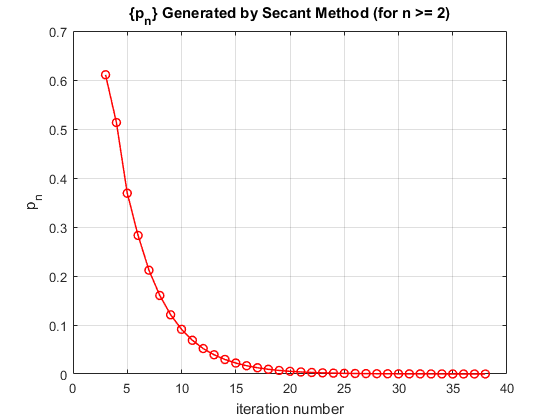
\includegraphics{secant.png}\\\\
	I also got the following from the console. Thus the solution is \boxtex{$ 2.620\times 10^{-5} $}.
	\begin{verbatim}
	The solution using secant method is 2.619881e-05 at iteration #38
	\end{verbatim}\pagebreak
	
	\item [(b)]
	The resulting graph I got is \\
	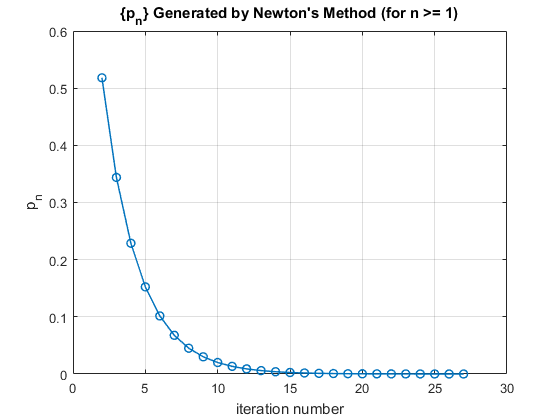
\includegraphics{newton.png}\\\\
	I also got the following from the console. Thus the solution is \boxtex{$ 1.357\times 10^{-5} $}.
	\begin{verbatim}
	The solution of Newton's method is 1.356836e-05 at iteration #27
	\end{verbatim}\pagebreak
	
\section*{Code for Question 5}
The following matlab codes are used.\\
\begin{verbatim}
% % MATH 151A HOMEWORK1 
% % QUESTION 5
% % Wang, Zheng

%%%%%%%%%%%%%%%%%%%%%%%%%%%%%%%%%%%%%%%%%%%%%%%%
%  Secant Method to solve f(x) = sin(x)-x = 0  
%%%%%%%%%%%%%%%%%%%%%%%%%%%%%%%%%%%%%%%%%%%%%%%%
% initialize
i = 2;
p0 = pi/4;
p1 = 3*pi/8;
q0 = f(p0);
q1 = f(p1);
arr_p = [];
arr_it = [];

% Set the max iteration number
N = 10000;

% Set the tolerance
TO = 10^(-5);


%iteration
while i <= N
    p = p1 - q1*(p1-p0)/(q1-q0);
    % stopping condition
    if abs(p - p1) < TO
        fprintf('The solution using secant method is %e at iteration #%d\n', p, i)
        break;
    end
    i = i+1;
    p0 = p1;
    q0 = q1;
    p1 = p;
    q1 = f(p);
    arr_p = [arr_p p];
    arr_it = [arr_it i];
end

% output the failure message if needed
if i > N
fprintf('Secant Method failed after %d iteration, the value found is %e\n',N, p)
end

% plot the graph
figure;
plot(arr_it, arr_p, 'o-r', 'Linewidth', 1.1);
title('\{p_n\} Generated by Secant Method (for n >= 2)');
xlabel('iteration number')
ylabel('p_n')
grid on;

%%%%%%%%%%%%%%%%%%%%%%%%%%%%%%%%%%%%%%%%%%%%%%%%%
%  Newton's Method to solve f(x) = sin(x)-x = 0
%%%%%%%%%%%%%%%%%%%%%%%%%%%%%%%%%%%%%%%%%%%%%%%%%
% initialize
i = 1;
p0 = pi/4;
q0 = f(p0);
d0 = fprim(p0);
arr_p = [];
arr_it = [];


% Set the max iteration number
N = 10000;

% Set the tolerance
TO = 10^(-5);

%iteration
while i <= N
    p = p0 - q0/d0;
    if abs(p - p0) < TO
        fprintf('The solution of Newton''s method is %e at iteration #%d\n', p, i)
        break;
    end
    i = i+1;
    p0 = p;
    arr_p = [arr_p p0];
    arr_it = [arr_it i];
    q0 = f(p0);
    d0 = fprim(p);
end

% output the failure message if needed
if i > N
fprintf('Newton''s Method failed after %d iteration, the value found is %e\n',N, p)
end

% plot the graph
figure;
plot(arr_it, arr_p, 'o-', 'Linewidth', 1.1);
title('\{p_n\} Generated by Newton''s Method (for n >= 1)');
xlabel('iteration number')
ylabel('p_n')
grid on;

% % function declaration
function y = f(x)
    y = sin(x) - x;
end

function y = fprim(x)
    y = cos(x) - 1;
end
\end{verbatim}
	
\end{itemize}
	




\end{document}